\documentclass[../root.tex]{subfiles}

\usepackage[export]{adjustbox}

\begin{document}

\chapter{
  Data-Efficient Model Learning for Model Predictive Control with
  Jacobian-Regularized Dynamic Mode Decomposition
} \label{chap:jdmd}
\chaptermark{JDMD}

\lettrine{W}e present a data-efficient algorithm for learning models for model-predictive
control (MPC). Our approach, Jacobian-Regularized DMD (JDMD), offers improved
sample efficiency over traditional Koopman approaches based on Dynamic-Mode
Decomposition (DMD) by leveraging Jacobian  information from an approximate
prior model of the system, and improved tracking performance over traditional
model-based MPC. We demonstrate JDMD's ability to quickly learn bilinear
Koopman dynamics representations across several realistic examples in
simulation, including a perching maneuver for a fixed-wing aircraft with an
experimentally derived high-fidelity physics model.   In all cases, we show
that the models learned by JDMD provide superior tracking and generalization
performance in the presence of significant model mismatch within a
model-predictive control framework,  when compared to the approximate prior
models used in training and models learned by  standard extended DMD.

\section{Introduction}

In recent years, both model-based optimal-control
\cite{farshidian_Efficient_2017, kuindersma_Efficiently_2014, bjelonic_WholeBody_2021, subosits_Racetrack_2019}
and data-driven
reinforcement-learning methods \cite{karnchanachari_Practical_2020,li_Reinforcement_2021}
 have
demonstrated impressive successes on complex, nonlinear robotic systems.
However, both approaches suffer from inherent drawbacks: Data-driven methods
often require extremely large amounts of data and fail to generalize outside of
the domain or task on which they were trained. On the other hand, model-based
methods require an accurate model of the system to achieve good performance. In
many cases, high-fidelity models can be too difficult to construct from first
principles or too computationally expensive to be of practical use. However,
low-order approximate models that can be evaluated cheaply at the expense of
controller performance are often available. With this in mind, we seek a middle
ground between model-based and data-driven approaches in this work. 

We propose a method for learning bilinear Koopman models of nonlinear dynamical
systems for use in model-predictive control that leverages \changed{derivative}
information from an approximate prior dynamics model of the system in the
training process.  \changed{Given the increased availability of differentiable
simulators \cite{howell_Dojo_2022,todorov_MuJoCo_2012}, this approximate
derivative information is readily available for many systems of interest.} Our
new algorithm builds on extended Dynamic Mode Decomposition (EDMD), which learns
Koopman models from trajectory data
\cite{meduri_BiConMP_2022,bruder_Advantages_2021,korda_Linear_2018,
folkestad_Episodic_2020,suh_Surprising_2020}, by adding a derivative
regularization term based on derivatives computed from a prior model.  We show
that this new algorithm, Jacobian-regularized Dynamic Mode Decomposition (JDMD),
can learn models with dramatically fewer samples than EDMD, even when the prior
model differs significantly from the true dynamics of the system.  We also
demonstrate the effectiveness of these learned models in a model-predictive
control (MPC) framework.
%on these systems when the learned bilinear system is linearized and projected
%back into the original state space.
The result is a fast, robust, and sample-efficient pipeline for quickly training
a model that can outperform \changed{MPC controllers using the approximate
analytical model as well models learned using both traditional Koopman
approaches and multi-layer perceptrons (MLPs).} \changed{While our proposed
Koopman-based approached is significantly more sample efficient, we also
demonstrate the utility of incorporating gradient information for learning a
simple model using a two-layer MLP}.
%To learn these bilinear representations, we also propose a numerical technique
%that allows for large systems to be trained while limiting the peak memory
%required to solve the least-squares problem.

Our work is most closely related to the recent work of Folkestad et. al.
\cite{folkestad_Koopman_2021,folkestad_Episodic_2020,folkestad_Extended_2020,folkestad_KoopNet_2022}
which learn bilinear models and apply nonlinear model-predictive control
directly on the learned bilinear dynamics. Other recent works have combined
linear Koopman models with model-predictive control \cite{korda_Linear_2018} and
Lyapunov control techniques with bilinear Koopman
\cite{narasingam_Datadriven_2022}. Our contributions are:

\begin{itemize}
  \item A novel extension to extended dynamic mode decomposition, called JDMD, that
  incorporates gradient information from an approximate analytic model
  
  \item A recursive, batch QR algorithm for solving the least-squares problems that arise 
  when learning bilinear dynamical systems using DMD-based algorithms, including JDMD and EDMD
  
%   \item A simple linear MPC control technique for learned bilinear control systems that is
%   computationally efficient and, when combined with JDMD, requires very little training data
%   to achieve good performance
\end{itemize}

The remainder of the paper is organized as follows: In Section
\ref{sec:Preliminaries/Background} we provide some background on the application
of Koopman operator theory to controlled dynamical systems and review some
related works.  Section \ref{sec:jdmd} then describes the proposed JDMD
algorithm.  In Section \ref{sec:rls} we outline a memory-efficient technique for
solving the large, sparse linear least-squares problems that arise when applying
JDMD and other DMD-based algorithms.  
% Next, in Section \ref{sec:projected_mpc}, we propose an efficient
% model-predictive control technique that utilizes the learned bilinear models
% produced by JDMD.  
Section \ref{sec:results} then provides simulation results and analysis of the
proposed algorithm applied to control tasks on a cartpole, a quadrotor, and a
small foam airplane \changed{with an experimentally determined aerodynamics
model}, all subject to significant model mismatch.  \changed{It also includes a
comparison of the current approach to model-learning via a multi-layer
perceptron, for the canonical cartpole problem.} In Section
\ref{sec:limitations} we discuss the limitations of our approach, followed by
some concluding remarks in Section \ref{sec:koopman_conclusion}.

\section{Background and Related Work} \label{sec:Preliminaries/Background}

\subsection{Koopman Operator Theory}

The theoretical underpinnings of the Koopman operator and its application to
dynamical systems has been extensively studied 
\cite{fasel_SINDy_2021,proctor_Generalizing_2018,bruder_Advantages_2021,williams_Data_2015,surana_Koopman_2016}
Rather than describe the theory in detail, we highlight the key concepts
employed by the current work and refer the reader to the existing literature on
Koopman theory for further details.

We start by assuming a controlled, nonlinear, discrete-time dynamical system,
\begin{equation} \label{eq:discrete_dynamics} 
  x^+ = f(x, u), 
\end{equation} 
where $x \in \mathcal{X} \subseteq \R^{N_x}$ is the state vector, $u_k \in
\R^{N_u}$ is the control vector, and $x^+$ is the state at the next time step.
\changed{Assuming the dynamics are control-affine, the nonlinear
finite-dimensional system \eqref{eq:discrete_dynamics} can be represented
\emph{exactly} by an infinite-dimensional bilinear system through the Koopman
canonical transform \cite{surana_Koopman_2016}. This bilinear Koopman model follows the
form,}
\begin{equation} \label{eq:bilinear_dynamics}
  y^+ = A y + B u + \sum_{i=1}^m u_i C_i y = g(y,u) ,
\end{equation}
where $y = \phi(x)$ is a nonlinear mapping from the finite-dimensional state
space $\mathcal{X}$ to the infinite-dimensional Hilbert space of
\textit{observables} $\mathcal{Y}$.  In practice, we approximate
\eqref{eq:bilinear_dynamics} by restricting $\mathcal{Y}$ to be a
finite-dimensional vector space, in which case $\phi$ becomes a
finite-dimensional nonlinear function of the state variables, \changed{which can
be either chosen heurstically based on domain expertise, or learned
\cite{folkestad_Extended_2020,folkestad_KoopNet_2022,li_Extended_2017}}.

Intuitively, $\phi$ ``lifts'' our state $x$ into a higher dimensional space
$\mathcal{Y}$ where the dynamics are approximately (bi)linear, effectively
trading dimensionality for (bi)linearity. Similarly, we can perform an
``unlifting'' operation by projecting a lifted state $y$ back into the original
state space $\mathcal{X}$. In this work, \changed{since we embed the original
state within the nonlinear mapping 
\cite{bruder_Advantages_2021,folkestad_Koopman_2021,mamakoukas_Local_2019,huang_Feedback_2018,ma_Optimal_2019}
}, $\phi$ is constructed in such a way that this unlifting is linear:
\begin{equation}
	x = G y.
\end{equation}
\changed{We note that our proposed method does not rely on this assumption: any
mapping could be used. The problem of finding an optimal mapping is itself a
major area of research, and many recent studies have focused on jointly learning
both the model and the mapping
\cite{folkestad_Extended_2020,folkestad_KoopNet_2022,wang_Deep_2021,kaiser_Datadriven_2021,
li_Extended_2017}.  While clearly advantageous, learning an optimal embedding is
orthogonal to the main focus of the current paper, which focuses on a
straightforward way of incorporating analytical derivative information from an
approximate model, which is equally applicable whether the embedding function is
learned or chosen heuristically.  The mappings in the current work are chosen
heuristically based on problem insight and experience.}

\subsection{Extended Dynamic Mode Decomposition} \label{sec:edmd}

A lifted bilinear system of the form \eqref{eq:bilinear_dynamics} can be learned
from $P$ samples of the system dynamics $(x_j^+,x_j,u_j)$ using Extended Dynamic
Mode Decomposition (EDMD) \cite{williams_Data_2015,folkestad_Koopman_2021}. We
first define the following data matrices:
\begin{equation}
  Z_{1:P} = \begin{bmatrix}
    y_1         & y_2         & \dots  & y_P          \\
    u_1         & u_2         & \dots  & u_P          \\
    u_{1,1} y_1 & u_{2,1} y_2 & \dots  & u_{P,1} y_P  \\
    \vdots      & \vdots      & \ddots & \vdots       \\
    u_{1,m} y_1 & u_{2,m} y_2 & \dots  & u_{P,m} y_P  \\
  \end{bmatrix}, \quad 
  Y_{1:P}^+ = \begin{bmatrix}
    y_1^+         & y_2^+         & \dots  & y_P^+    \\
  \end{bmatrix},
\end{equation}
We then concatenate all of the model coefficient matrices as follows:
\begin{equation} \label{eq:E_matrixdef}
  E = \begin{bmatrix} A & B & C_1 & \dots & C_m \end{bmatrix} \in \R^{N_y \times N_z},
\end{equation}
The model learning problem can then be written as the following linear least-squares problem:

\begin{align} \label{opt:edmd}
  \underset{E}{\text{minimize}} \; \norm{E Z_{1:P} - Y_{1:P}^+}_2^2
\end{align}

\changed{EDMD is closely related to classical feature-based machine learning
approaches like the ``kernel trick'' used in support vector machines
\cite{kutz_Dynamic_2016}, but extends these ideas to bilinear models of
controlled dynamical systems.}


%%%%%%%%%%%%%%%%%%%%%%%%%%%%%%%%%%%%%%%%%%%%%%%%%%%%%%%%%%%%%%%%%%%%%%%%%%%%%%%%%%%%%%%%%%
% Methodology
%%%%%%%%%%%%%%%%%%%%%%%%%%%%%%%%%%%%%%%%%%%%%%%%%%%%%%%%%%%%%%%%%%%%%%%%%%%%%%%%%%%%%%%%%%
\section{Jacobian-Regularizated Dynamic Mode Decomposition} \label{sec:jdmd}

We now present JDMD as a straightforward adaptation of the original EDMD algorithm described
in Section \ref{sec:edmd}. Given $P$ samples of the dynamics $(x_i^+, x_i, u_i)$, and an
approximate discrete-time dynamics model,
\begin{equation}
  x^+ = \tilde{f}(x,u),
\end{equation}
we can evaluate the Jacobians of our approximate model $\tilde{f}$ at each of the sample
points: $\tilde{A}_i = \pdv{\tilde{f}}{x}, \tilde{B}_i = \pdv{\tilde{f}}{u}$. After
choosing a nonlinear mapping $\phi : \R^{N_x} \mapsto \R^{N_y}$ our goal is to find a
bilinear dynamics model \eqref{eq:bilinear_dynamics} that matches the Jacobians of our
approximate model, while also matching our dynamics samples. We accomplish this by 
penalizing differences between the Jacobians of our learned bilinear model with respect to 
the original states $x$ and controls $u$, and the Jacobians we expect from our analytical 
model. These \textit{projected Jacobians} are calculated by differentiating through the 
\textit{projected dynamics}:
\begin{equation} \label{eq:projected_dynamics}
  x^+ = G \left( A \phi(x) + B u + \sum_{i=1}^m u_i C_i \phi(x) \right)  = \bar{f}(x,u).
\end{equation}
Differentiating \eqref{eq:projected_dynamics} with respect to $x$ and $u$ gives us
\begin{subequations} \label{eq:projected_jacobians}
  \begin{align}
    \bar{A}_j &= \pdv{\hat{f}}{x}\left(x_j,u_j\right) 
    = G \left(A + \sum_{i=1}^m u_{j,i} C_i \right) \Phi(x_j)
    %   = G A_j^x \phi(x_j)
    = G E \hat{A}(x_j,u_j) = G E \hat{A}_j \\
    \bar{B}_j &= \pdv{\hat{f}}{u}\left(x_j,u_j\right) 
    = G \Big(B + \begin{bmatrix} C_1 x_j & \dots & C_m x_j \end{bmatrix} \Big)
    %   = G B_j^u
    = G E \hat{B}(x_j,u_j) = G E \hat{B}_j
  \end{align}
\end{subequations}
where $\Phi(x) = \pdv*{\phi}{x}$ is the Jacobian of the nonlinear map $\phi$, and
\begin{equation}
  \hat{A}(x,u) =  \begin{bmatrix} 
    I_{N_y} \\ 0 \\ u_1 I_{N_y} \\ u_2 I_{N_y} \\ \vdots \\ u_m I_{N_y} 
  \end{bmatrix} \Phi(x) \in \R^{N_z \times N_x}, \quad
  \hat{B}(x,u) = \begin{bmatrix} 
    0 \\ 
    I_{N_u} \\ 
    [\phi(x) \; 0 \; ... \; 0] \\
    [0 \; \phi(x) \; ... \; 0] \\
    \vdots \\
    [0 \; 0 \; ... \; \phi(x)] \\
  \end{bmatrix} \in \R^{N_z \times N_u}.
\end{equation}

We then solve the following linear least-squares problem:
\begin{align} \label{opt:jdmd}
  \underset{E}{\text{minimize}} \;\; 
    (1-\alpha) \norm{E Z_{1:P} - Y_{1:P}^+}_2^2 + 
        \alpha \sum_{j=1}^P \left( 
          \norm{G E \hat{A}_j - \tilde{A}_j}_2^2 + 
          \norm{G E \hat{B}_j - \tilde{B}_j}_2^2 \right)
\end{align}

The resulting linear least-squares problem has $(N_y + N_x^2 + N_x \cdot N_u) \cdot P$ rows
and $N_y \cdot N_z$ columns. Given that the number of rows in this problem grows
quadratically with the state dimension, solving this problem can be challenging from a
computational perspective. In the Section \ref{sec:rls}, we propose an algorithm for solving
these problems without needing to move to a distributed-memory setup in order to solve these
large linear systems. The proposed method also provides a straightforward way to approach
incremental updates to the bilinear system, where the coefficients could be efficiently
learned ``live'' while the robot gathers data by moving through its environment.

% If we define $\hat{A}_j \in
% \R^{N_x \times N_x}$ and $\hat{B}_j \in \R^{N_x \times N_u}$ to be the Jacobians of our
% bilinear dynamics model, projected back into the original state space (a formal definition
% of these terms will be provided in a few paragraphs), our objective is to find the
% matrices that parameterize our bilinear dynamics model, $A \in \R^{N_y \times N_y},B \in
% \R^{N_y \times N_u}$, and $C_{1:m} \in \R^{N_u} \times \R^{N_y \times N_y}$, that minimize
% the following objective:

% \begin{equation} \label{eq:lls_objective}
%   (1- \alpha) \sum_{j=1}^P \norm{\hat{y}_j - y_j^+}_2^2 + 
%   \alpha  \sum_{j=1}^P \norm{\hat{A}_j - \tilde{A}_j}_2^2 + 
%   \norm{\hat{B}_j - \tilde{B}_j}_2^2 
% \end{equation}
% where $\hat{y}_j^+ = g\left(\phi(x_j), u_j\right)$ is the output of our bilinear dynamics
% model, and $y_j^+ = \phi(x_j^+)$ is the actual lifted state (i.e. observables) at the next
% time step. Note that $\hat{y}_j$, $\hat{A}_j$, and $\hat{B}_j$ are all implicitly
% functions of the model parameters $A$, $B$, and $C_{1:m}$ we're trying to learn.

% While not immediately apparent, we can minimize \eqref{eq:lls_objective} using linear
% least-squares, using techniques similar to those used previously in the literature
% \cite{Folkestad2021}.

% To start, we combine all the data we're trying to learn into a single matrix:
% \begin{equation}
%   E = \begin{bmatrix} A & B & C_1 & \dots & C_m \end{bmatrix} \in \R^{N_y \times N_z},
% \end{equation}
% where $N_z = N_y + N_u + N_y \cdot N_u$.  We now rewrite the terms in
% \eqref{eq:lls_objective} in terms of $E$. By defining the vector 
% \begin{equation}
%   z = \begin{bmatrix} y^T & u^T & u_1 y^T & \dots & u_m y^T \end{bmatrix} \in \R^{N_z},
% \end{equation}
% we can write down 
% the output of our bilinear dynamics \eqref{eq:bilinear_dynamics} as 
% \begin{equation} \label{eq:bilinear_dynamics_z}
%   \hat{y}^+ = E z.
% \end{equation}
% The previously-mentioned projected Jacobians of our bilinear model, $\hat{A}$ and
% $\hat{B}$, are simply the Jacobians of the bilinear dynamics in terms of the original
% state. We obtain these dynamics by ``lifting`` the state via $\phi$ and then projecting
% back onto the original states using $G$:
% \begin{equation} \label{eq:projected_dynamics}
%   x^+ = G \left( A \phi(x) + B u + \sum_{i=1}^m u_i C_i \phi(x) \right)  = \hat{f}(x,u) 
% \end{equation}
% Differentiating these dynamics gives us our projected Jacobians:
% \begin{subequations} \label{eq:projected_jacobians}
%   \begin{align}
%     \hat{A}_j &= \pdv{\hat{f}}{x}\left(x_j,u_j\right) 
%     = G \left(A + \sum_{i=1}^m u_{j,i} C_i \right) \Phi(x_j)
%     %   = G A_j^x \phi(x_j)
%     = G E \bar{A}(x_j,u_j) = G E \bar{A}_j \\
%     \hat{B}_j &= \pdv{\hat{f}}{u}\left(x_j,u_j\right) 
%     = G \Big(B + \begin{bmatrix} C_1 x_j & \dots & C_m x_j \end{bmatrix} \Big)
%     %   = G B_j^u
%     = G E \bar{B}(x_j,u_j) = G E \bar{B}_j
%   \end{align}
% \end{subequations}
% where $\Phi(x) = \pdv*{\phi}{x}$ is the Jacobian of the nonlinear map $\phi$, and
% \begin{equation}
%   \bar{A}(x,u) =  \begin{bmatrix} 
%     I \\ 0 \\ u_1 I \\ u_2 I \\ \vdots \\ u_m I 
%   \end{bmatrix} \in \R^{N_z \times N_x}, \quad
%   \bar{B}(x,u) = \begin{bmatrix} 
%     0 \\ 
%     I \\ 
%     [x \; 0 \; ... \; 0] \\
%     [0 \; x \; ... \; 0] \\
%     \vdots \\
%     [0 \; 0 \; ... \; x] \\
%   \end{bmatrix} \in \R^{N_z \times N_u}.
% \end{equation}
% Note we define $\bar{A}_j = \bar{A}(x_j,u_j)$, $\bar{B}_j = \bar{B}(x_j,u_j)$ to lighten 
% the notation, but want to emphasize that these terms are all purely functions of the input
% data.

% Substituting \eqref{eq:bilinear_dynamics_z} and \eqref{eq:projected_jacobians} into
% \eqref{eq:lls_objective}, we can rewrite our LLS problem as:
% \begin{align}
%   \underset{E}{\text{minimize}} \;\; 
%   \sum_{j=0}^P
%   (1-\alpha) \norm{E z_j - y_j^+}_2^2 + 
%   \alpha  \norm{G E \bar{A}_j - \tilde{A}_j}_2^2 + 
%   \alpha  \norm{G E \bar{B}_j - \tilde{B}_j}_2^2 
% \end{align}
% which is equivalent to
% \begin{align} \label{opt:lls_matrices}
%   \underset{E}{\text{minimize}} \;\; 
%   (1-\alpha) \norm{E \mathbf{Z_{1:P}} - \mathbf{Y^+_{1:P}} }_2^2 + 
%   \alpha  \norm{G E \mathbf{\bar{A}_{1:P}} - \mathbf{\tilde{A}_{1:P}}}_2^2 + 
%   \alpha  \norm{G E \mathbf{\bar{B}_{1:P}} - \mathbf{\tilde{B}_{1:P}}}_2^2
% \end{align}
% where $\mathbf{Z_{1:P}} \in \R^{N_z \times P} = [z_1 \; z_2 \; ... \; z_P]$ horizontally
% concatenates all of the samples (equivalent definition for 
% $\mathbf{Y^+_{1:P}} \in \R^{N_y \times P}$, 
% $\mathbf{\bar{A}_{1:P}} \in \R^{N_z \times N_x \cdot P}$, 
% $\mathbf{\tilde{A}_{1:P}} \in \R^{N_z \times N_x \cdot P}$,
% $\mathbf{\bar{B}_{1:P}} \in \R^{N_z \times N_u \cdot P}$, and 
% $\mathbf{\tilde{B}_{1:P}} \in \R^{N_z \times N_u \cdot P}$ ).

% We can rewrite \eqref{opt:lls_matrices} in standard form using the ``vec trick''
% \begin{equation} \label{eq:vectrick}
%   \text{vec}(A X B) = (B^T \otimes A) \text{vec}(X)
% \end{equation}
% where $\text{vec}(A)$ stacks the columns of $A$ into a single vector.

% Setting $E$ in \eqref{opt:lls_matrix} equal to $X$ in \eqref{eq:vectrick}, we get
% \begin{align} \label{opt:lls_matrix}
%   \underset{E}{\text{minimize}} \;\;  
%   \norm{
%   \begin{bmatrix}
%     (1-\alpha)\cdot(\mathbf{Z_{1:P}})^T \otimes I_{N_y} \\
%     \alpha\cdot(\mathbf{\bar{A}_{1:P}})^T \otimes G \\
%     \alpha\cdot(\mathbf{\bar{G}_{1:P}})^T \otimes G \\
%   \end{bmatrix}
%   \text{vec}(E)
%   +
%   \begin{bmatrix}
%     (1-\alpha)\cdot\text{vec}(\mathbf{Y^+_{1:P}}) \\
%     \alpha\cdot\text{vec}(\mathbf{\tilde{A}_{1:P}}) \\
%     \alpha\cdot\text{vec}(\mathbf{\tilde{G}_{1:P}})
%   \end{bmatrix}
%   }_2^2
% \end{align}
% such that the matrix of coefficients has $(N_y + N_x^2 + N_x \cdot N_u) \cdot P$ rows and 
% $N_y \cdot N_z$ columns. We obtain the data for our bilinear model 
% \eqref{eq:bilinear_dynamics} by solving this large, sparse linear least-squares 
% problem.

%%%%%%%%%%%%%%%%%%%%%%%%%%%%%%%%%%%%%%%%%%%%%%%%%%%%%%%%%%%%%%%%%%%%%%%%%%%%%%%%%%%%%%%%%%%%
\section{Efficient Recursive Least Squares} \label{sec:rls}
%%%%%%%%%%%%%%%%%%%%%%%%%%%%%%%%%%%%%%%%%%%%%%%%%%%%%%%%%%%%%%%%%%%%%%%%%%%%%%%%%%%%%%%%%%%%
In its canonical formulation, a linear least squares problem can be represented as the
following unconstrained optimization problem:
\begin{align} \label{opt:lls}
  \min_x \|Fx - d\|_2^2.
\end{align}
We assume $F$ is a large, sparse matrix and that solving it directly using a QR or Cholesky
decomposition requires too much memory for a single computer. While solving \eqref{opt:lls}
using an iterative method such as LSMR \cite{fong_LSMR_2011} or LSQR \cite{paige_LSQR_1982}
 is possible,
we find that these methods do not work well in practice for solving \eqref{opt:jdmd} due to
ill-conditioning.  Standard recursive methods for solving these problems are able to process
the rows of the matrices sequentially to build a QR decomposition of the full matrix, but
also tend to suffer from ill-conditioning 
\cite{strobach_Recursive_1990,sayed_Recursive_2009,ghirnikar_Stable_1990}.

To overcome these issues, we propose an alternative recursive method. We solve
\eqref{opt:lls} by dividing up rows of $F$ into batches:
\begin{align} \label{eq:F_sum}
  F^T F = F_1^T F_1 + F_2^T F_2 + \ldots + F_N^T F_N.
\end{align}
The main idea is to maintain and update an upper-triangular Cholesky factor $U_i$ of the
first $i$ terms of the sum \eqref{eq:F_sum}. Given $U_i$, we can calculate $U_{i+1}$ using
the $\operatorname{QR}$ decomposition, as shown in \cite{howell_ALTRO_2019}
\begin{equation}
  U_{i+1} = \sqrt{U_i^TU_i + F_{i+1}^TF_{i+1}} = 
  \operatorname{QR_R}\bigg( \begin{bmatrix} {U_i} \\ {F_{i+1}} \end{bmatrix} \bigg),
\end{equation}
where $\operatorname{QR_R}$ returns the upper triangular matrix $R$ from the 
$\operatorname{QR}$ decomposition. For an efficient implementation, this function should be
an ``economy'' or ``Q-less'' $\operatorname{QR}$ decomposition 
% \cite{cite something (e.g.  Van Loan)}, 
since the $Q$ matrix is never needed.

We also handle regularization of the normal equations, equivalent to adding Tikhonov
regularization to the original least squares problem, during the base
case of our recursion. If we want to add an L2 regularization with weight $\lambda$, we
calculate $U_1$ as:

\begin{equation}
  U_1 =  \operatorname{QR_R}\bigg( 
  \begin{bmatrix} {F_1} \\ \sqrt{\lambda} I \end{bmatrix}.
  \bigg).
\end{equation}

\changed{Throughout the paper, the results presented for both EDMD and JDMD
correspond to the best-performing L2-regularization values for each algorithm to
ensure a fair comparison is made. We perform a sweep over a range of
L2-regularization values for each study, with MPC tracking error as the metric.}

% The final algorithm for solving a least squares problem in a recursive-batch fashion is
% described in algorithm \ref{alg:rlsqr}. This algorithm can be modified to handle L2
% regularized least squares problems by simply replacing line 2 of algorithm \ref{alg:rlsqr}
% with $U\leftarrow \operatorname{QR_R}(\operatorname{vcat}(F_1,\sqrt{\rho}I))$, where $\rho$
% is the regularizer. 
% \begin{algorithm} 
%   \begin{algorithmic}[1]
%     \caption{Recursive Batch Least Squares with QR}\label{alg:rlsqr}
%     \State \textbf{input} $F,\,d$  \Comment{problem data}
%     \State $U \leftarrow \operatorname{QR_R}(\operatorname{vcat}(F_1,\sqrt{\rho}I))$ \Comment{form initial upper-triangular square-root}
%     \State $b \leftarrow F_1^Td_1$ \Comment{form initial right hand side vector}
%     \For{$i = 2:N$}
%     % 		\State $U \leftarrow \operatorname{QR_R}([U^T \, A_i^T]^T) $ 
%     \State $U \leftarrow \operatorname{QR_R}(\operatorname{vcat}(U,F_i)) $ \Comment{update square-root with new batch}
%     \State $b \leftarrow b + F_i^Td_i$ \Comment{update right hand side with new batch}
%     \EndFor
%     \State \textbf{output} \,$x \leftarrow U^{-1}U^{-T}b$ \Comment{forward and backwards substitution to solve for $x$}
%   \end{algorithmic}
% \end{algorithm}

% \section{Projected Bilinear MPC} \label{sec:projected_mpc}

% We propose a simple approach to model-predictive control for the bilinear systems learned
% using either classic EDMD or the proposed JDMD approach. The key idea is to use the 
% projected Jacobians $\bar{A}$ and $\bar{B}$ in \eqref{eq:projected_jacobians}, effectively
% reducing the problem to a standard linear MPC problem in the original state space instead of
% the larger, lifted one.  In the all of the examples in the following section, our MPC
% controller solves the following convex Quadratic Program (QP):
% % \begin{mini}[2]
% %   {x_{1:N}, u_{1:N}}{\half x_N^T Q_N x_N + \frac \sum_{k=1}^{N-1} x_k^T Q_k x_k + u_k^T R_k u_k}{}{}
% % \end{mini}
% \begin{mini}
%   {x_{1:N}, u_{1:N-1}}{\half x_N^T Q_N x_N + \half \sum_{k=1}^{N-1} x_k^T Q_k x_k + u_k^T R_k u_k }{}{}
%   \addConstraint{x_{k+1} = \bar{A}_k x_k + \bar{B}_k u_k + d_k}{}
%   \addConstraint{x_1 = x_\text{init}}
% \end{mini}
% where here we define $x$ and $u$ to be the ``delta''  from the reference trajectory
% $\bar{x}_{1:N}$,
% $\bar{u}_{1:N-1}$. The affine dynamics term $d_k = f(\bar{x}_k, \bar{u}_k) - \bar{x}_{k+1}$
% allows for dynamically infeasible reference trajectories. The projected Jacobians can be
% efficiently calculated from the bilinear dynamics either offline or online, and since the
% problem dimension is the same size as the linear MPC problem for the original dynamics, it
% is no more expensive to compute. This formulation also makes it trivial to enforce
% additional control or path constraints, and 
% avoids the need to regularize or otherwise constrain the lifted states.

%%%%%%%%%%%%%%%%%%%%%%%%%%%%%%%%%%%%%%%%%%%%%%%%%%%%%%%%%%%%%%%%%%%%%%%%%%%%%%%%%%%%%%%%%%
% Results
%%%%%%%%%%%%%%%%%%%%%%%%%%%%%%%%%%%%%%%%%%%%%%%%%%%%%%%%%%%%%%%%%%%%%%%%%%%%%%%%%%%%%%%%%%
\section{Experimental Results} \label{sec:results}

This section presents the results of several simulation experiments to evaluate the
performance of JDMD.  For each simulated system we specify two models: a \textit{nominal}
model, which is simplified and contains both parametric and non-parametric model error, and
a \textit{true} model, which is used exclusively for simulating the system and evaluating
algorithm performance.

All models were trained by simulating the ``true'' system with a nominal
controller to collect data in the region of the state space relevant to the
task. A set of fixed-length trajectories were collected, each at a sample rate
of 20-25 Hz. The bilinear EDMD model was trained using the same approach
introduced by Folkestad and Burdick \cite{folkestad_Koopman_2021} \changed{When
applying MPC to the learned Koopman models, the projected Jacobians 
\eqref{eq:projected_jacobians} were used, since this projected system is much
more likely to be controllable than the lifted one and reduces the computational
complexity back to that of the nominal MPC controller. This results in a
nonlinear model in the original state space, which is linearized about the
reference trajectory to create a linear MPC controller.} All continuous dynamics
were discretized with an explicit fourth-order Runge Kutta integrator. Code for
all experiments is available at \url{https://github.com/bjack205/BilinearControl.jl}.

\subsection{Systems and Tasks}

\begin{figure}
    \begin{subfigure}{\linewidth}
        \centering
        \includegraphics[width=\textwidth]{koopman/perch_cropped.png}
        \caption{Expert perching demonstration, a high angle-of-attack maneuver that minimizes 
                velocity at the goal position with complex, post-stall aerodynamic forces}
        \label{fig:perch}
    \end{subfigure}
    \par\medskip
    \begin{subfigure}{.4\linewidth}
        \centering
        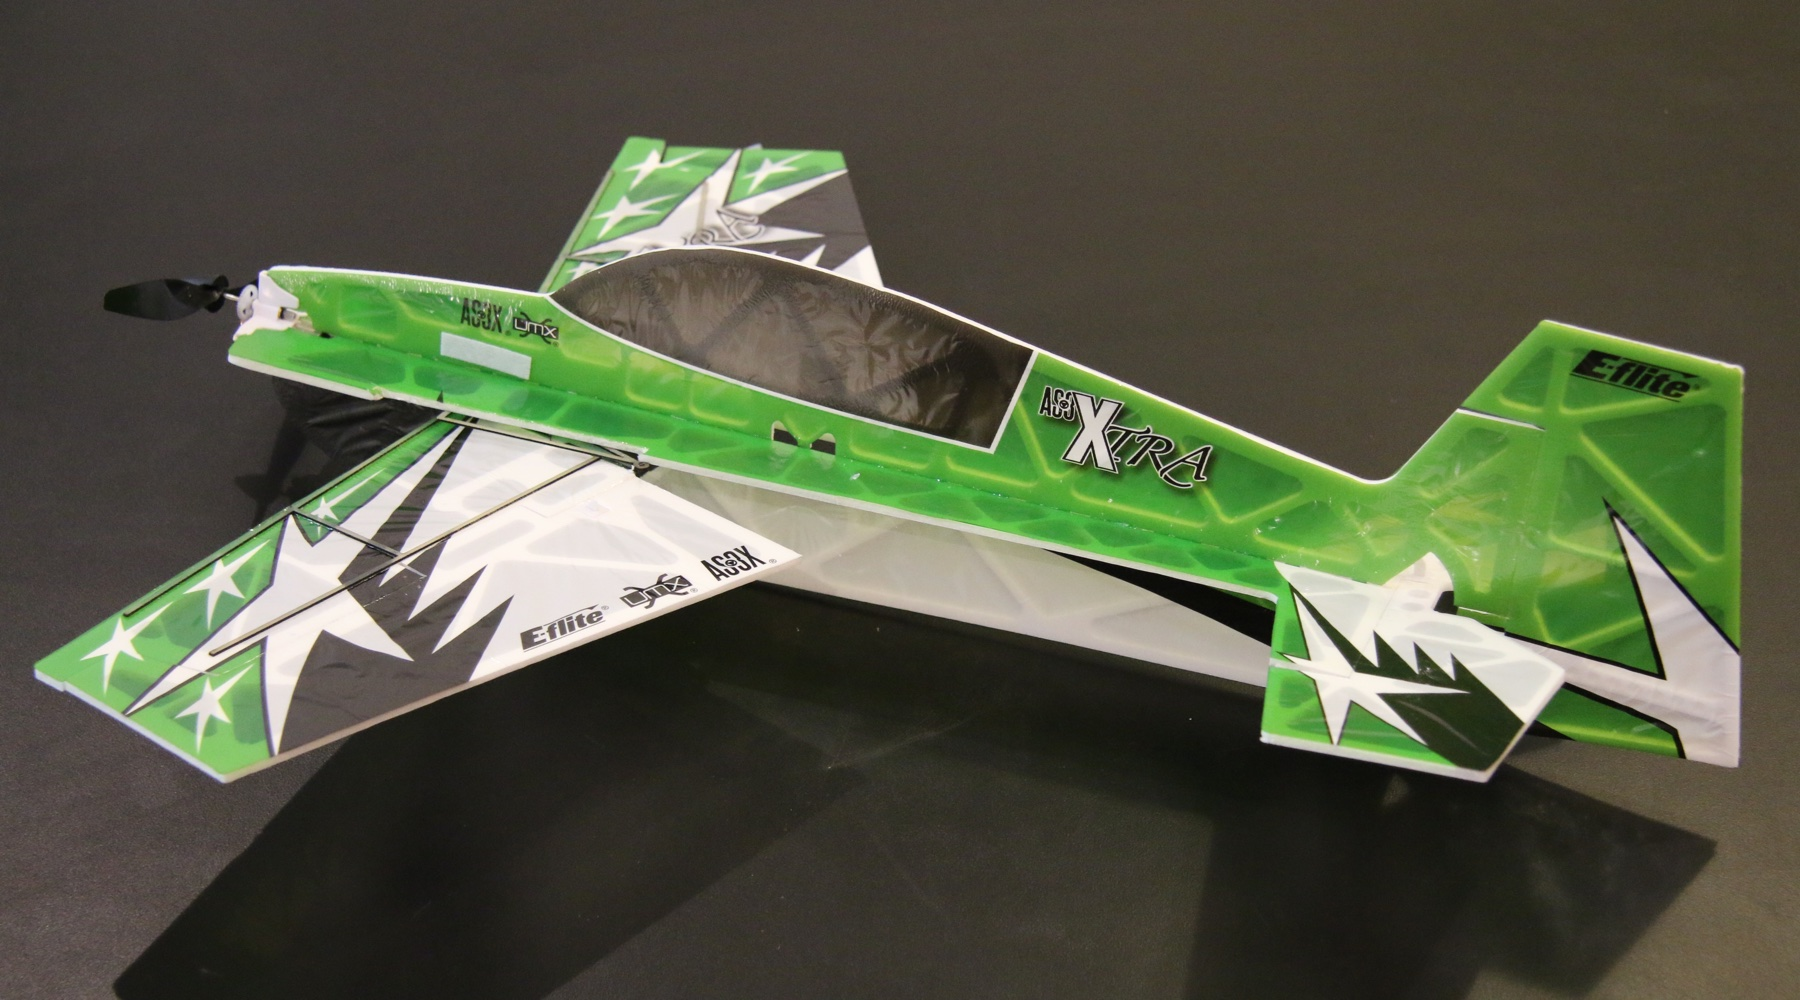
\includegraphics[height=3.1cm]{koopman/foamy/extra-sweep.jpg}
        \caption{E-Flite AS3Xtra airplane model used in hardware data collection}
        \label{fig:hw1}
    \end{subfigure}%
    \hfill
    \begin{subfigure}{.52\linewidth}
        \centering
        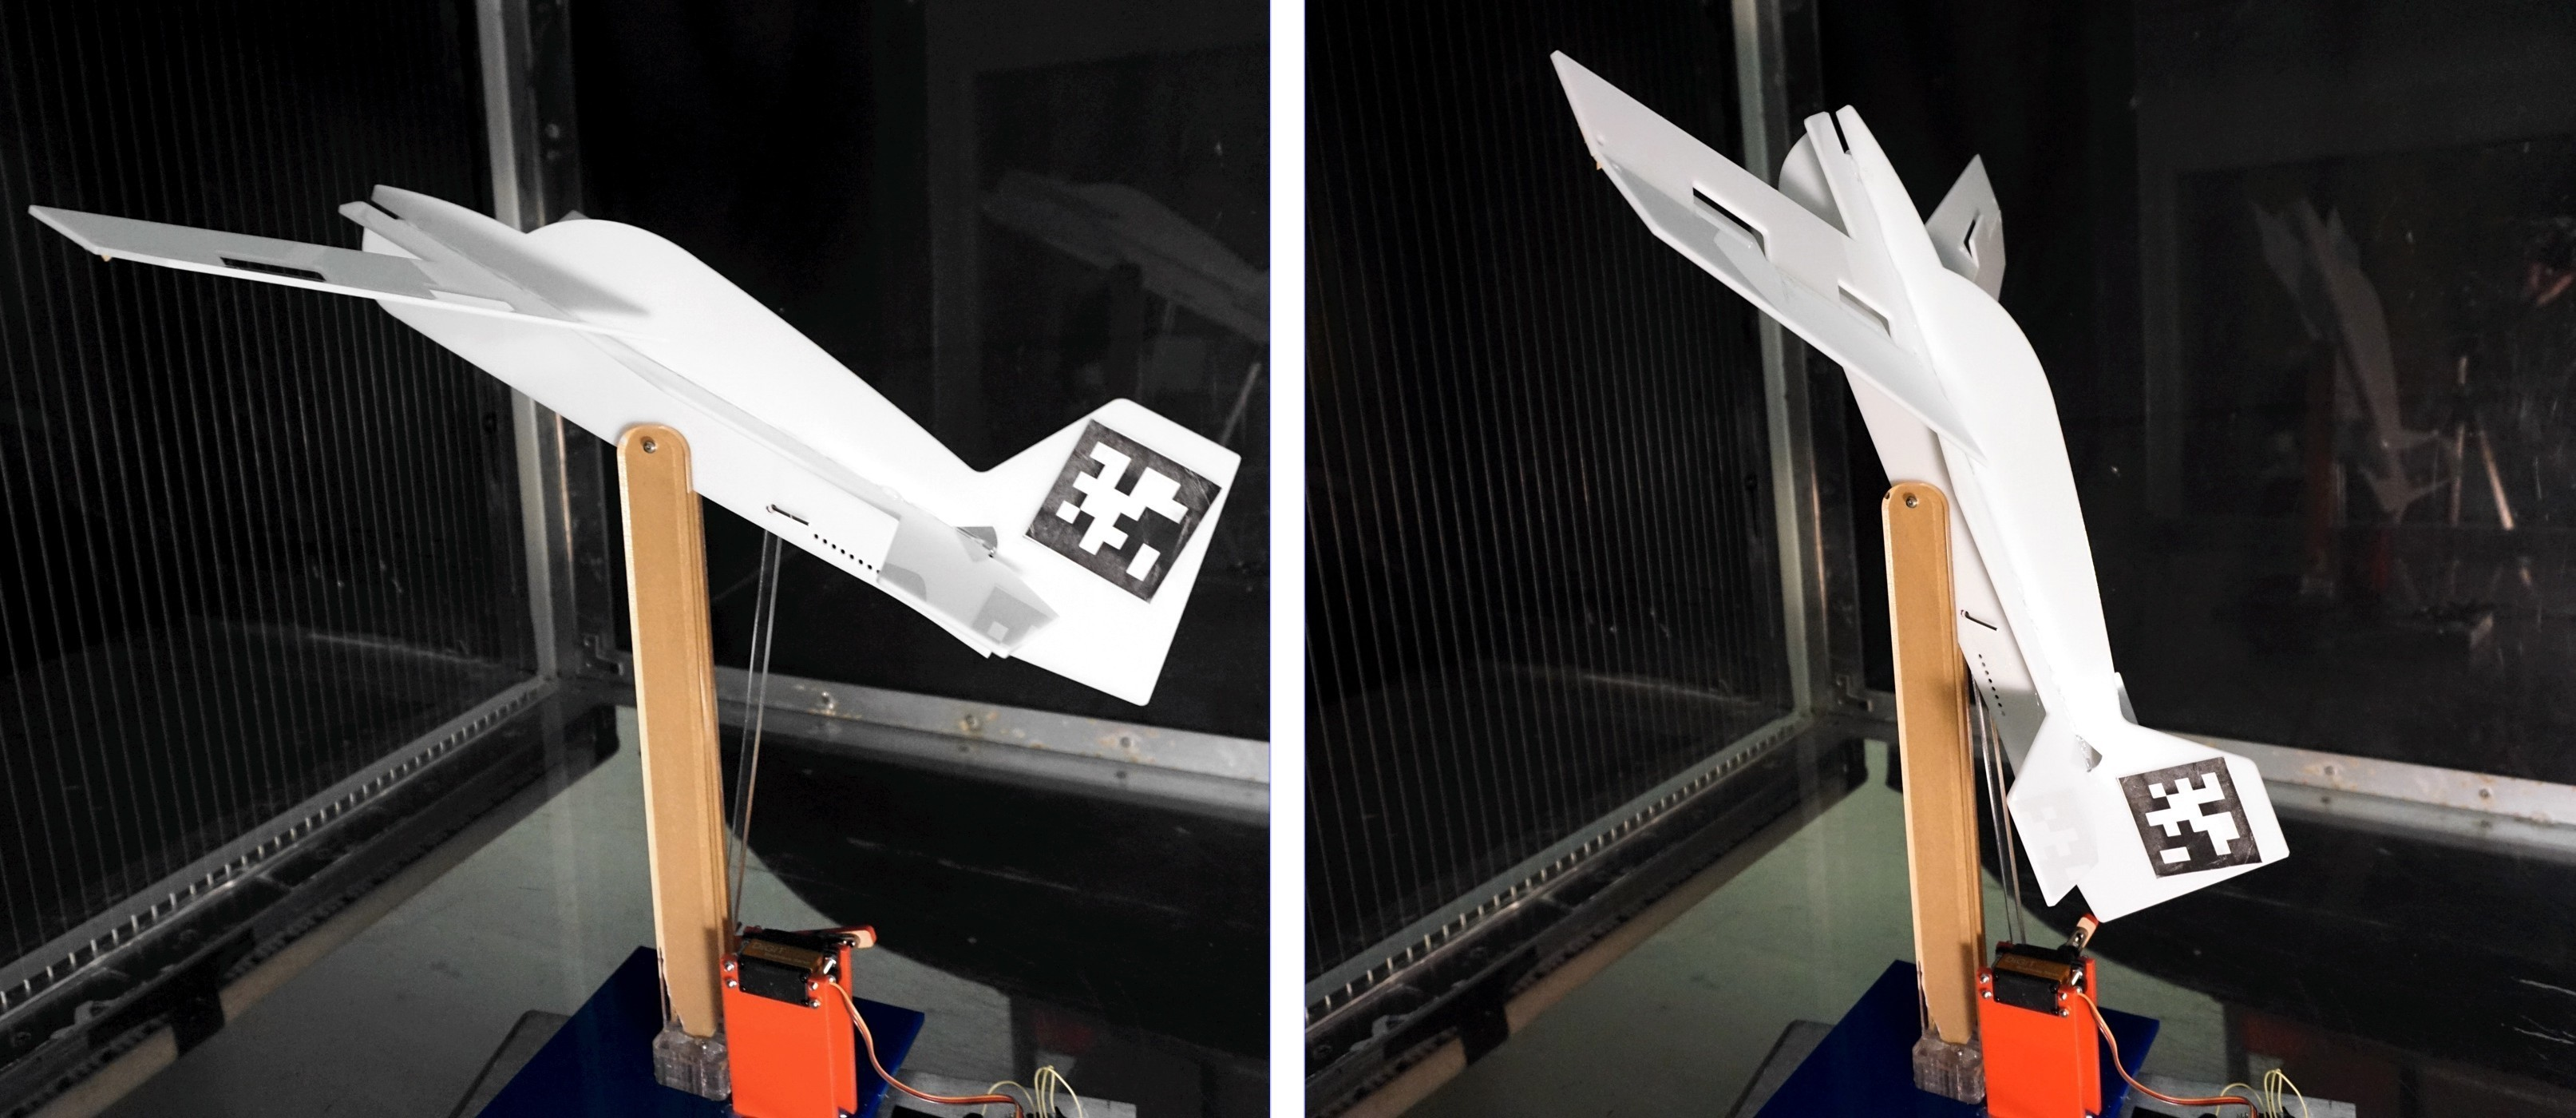
\includegraphics[height=3.1cm]{koopman/foamy/TestStand2&3.jpg}
        \caption{Experiment setup configurations for collecting flight data}
        \label{fig:hw2}
    \end{subfigure}\\[1ex]
    \caption{\changed{Complex dynamics of a perching fixed-wing airplane. High-angle-of-attack perching maneuvers (top) require the modeling of complex post-stall aerodynamic effects. The simulated aerodynamic forces were modeled as functions using flight data collected from real-world hardware experiments (bottom).}}
    \label{fig:test}
\end{figure}

% \begin{figure}{\linewidth}
%     \centering
%     \includegraphics[width=\textwidth]{perch_cropped.png}
%     \caption{Expert perching demonstration, a high angle-of-attack maneuver that minimizes 
%             velocity at the goal position}
%     \label{fig:perch}
% \end{figure}

\textbf{Cartpole:} We perform a swing-up task on a cartpole system. The \textit{true} model
includes Coulomb friction between the cart and the floor, viscous damping at both joints,
and a deadband in the control input that were not included in the \textit{nominal} model.
Additionally, the mass of the cart and pole model were altered by 20\% and 25\% with respect
to the nominal model, respectively.  The following nonlinear mapping was used when learning
the bilinear models: 
$$\phi(x) = [\, 1,\,
x,\, \sin(x),\, \cos(x),\, \sin(2x),\, \sin(4x),\, T_2(x),\, T_3(x),\, T_4(x)\, ] \in
\R^{33}$$, where $T_i(x)$ is a Chebyshev polynomial of the first kind of order $i$. 
All reference trajectories for the swing up task were generated using ALTRO 
\cite{howell_ALTRO_2019,jackson_ALTROC_2021}.

\textbf{Quadrotor:} We track point-to-point linear reference trajectories from
various initial conditions on both planar and full 3D quadrotor models. For both systems,
the \textit{true} model includes aerodynamic drag terms not included in the \textit{nominal}
model, as well as parametric error of roughly 5\% on the system parameters (e.g. mass, rotor
arm length, etc.). The planar model was trained using a nonlinear mapping of $\phi(x) = [\,
1,\, x,\, \sin(x),\, \cos(x),\, \sin(2x),\, T_2(x) ] \in \R^{25}$ while the full quadrotor
model was trained using a nonlinear mapping of $\phi(x) = [\, 1,\, x,\, T_2(x),\, \sin(p),\,
\cos(p),\, R^{T}v,\ v^{T}RR^{T}v,\, p \times v,\, p \times \omega,\, \omega \times \omega ]
\in \R^{44}$, where $p$ is the quadrotor's position, $v$ and $\omega$ are the translational
and angular velocities respectively, and $R$ is the rotation matrix.

\textbf{Airplane:} We perform a post-stall perching maneuver on a high-fidelity model of
a fixed-wing airplane. The perching trajectory is produced using trajectory optimization
(see Figure \ref{fig:perch}) and tracked using MPC. \changed{Perching involves flight at high
angles of attack, where the aerodynamic lift and drag forces are extremely complex and
difficult to model from first principles. We look to previous works where the simulated
aerodynamics were fitted using empirical data from in-person, wind-tunnel experiments
(see Figure \ref{fig:hw1} and \ref{fig:hw2}) before being demonstrated on hardware platforms
\cite{moore_Robust_2014,manchester_Variable_2017}.
The \textit{true} model includes the empirically-modeled,
nonlinear flight dynamics \cite{manchester_Variable_2017}, while the \textit{nominal}
model uses a simple flat-plate wing model with linear lift and quadratic drag coefficient
approximations.} The bilinear models use a 68-dimensional nonlinear mapping $\phi$ including
terms such as the rotation matrix (expressed in terms of a Modified Rodriguez Parameter),
powers of the angle of attack and side slip angle, the body frame velocity, various cross
products with the angular velocity, and some 3rd and 4th order Chebyshev polynomials
of the states.

% nonlinear mapping: $\phi(x) = [1, x, \text{vec}(R), v_\text{body}, v_\text{body}^T
% v_\text{body}, \sin(p), \alpha, \beta, \alpha^2, \beta^2, \alpha^3, \beta^3, p \times v, p
% \times \omega, \omega \times \omega, T_3(x), T_4(x) ] \in \R^{68}$, where $p \in \R^3$ is
% the position, $g \in \R^3$ is the attitude expressed as Modified Rodriguez Parameter, $v \in
% \R^3$ is the linear velocity in the world frame, $\omega \in \R^3$ is the angular velocity,
% $R \in \R^{3 \times 3}$ is the rotation matrix expressed in terms of $g$, $v_\text{body}$ is
% the velocity in the body frame, $\alpha$ is the angle of attack, and $\beta$ is the side
% slip angle.

%%%%%%%%%%%%%%%%%%%%%%%%%%%%%%%%%%%%%%%%%%%%%
\subsection{Sample Efficiency}
%%%%%%%%%%%%%%%%%%%%%%%%%%%%%%%%%%%%%%%%%%%%%

\changed{We compare the sample efficiency of several algorithms on the cartpole swing-up task in Fig. 
\ref{fig:sample_efficiency}, including a simple two-layer multi-layer perceptron trained using the a loss function
equivalent to \eqref{opt:jdmd} with $\alpha = 1$ (MLP) and $\alpha \in (0,1)$ (JMLP). For JMLP, $\alpha$ was 
monotonically decreased over time, in order to place more weight on the data as more data was used 
(red line in Fig. \ref{fig:cartpole_mlp}).
The derivatives of the model
with respect to the inputs are calculated automatically using backward propagation of the partial derivatives 
for usage in the loss function, resulting in second-order derivatives of the $\tanh$ activation functions when 
calculating the gradient with respect to the model parameters.
As shown, the proposed method achieves the best performance overall, and does so
with only two training trajectories. In comparison, traditional EDMD requires about 10 iterations to achieve 
consistent performance, whereas the MLP methods require hundreds of training trajectories. It's also important 
to note that by applying the proposed approach to an MLP we were 
able to dramatically improve both the performance and sample efficiency of the MLP-based approach.
Similar results were obtained for the airplane perching example (Fig. \ref{fig:airplane_sample_efficiency}),
where EDMD requires about 3x the number of samples (35 vs 10) compared to the proposed approach, and never achieves the same closed-loop performance.}
% We highlight the sample efficiency of the proposed algorithm compared to a multi-layer perceptron in Figure 
% \ref{fig:sample_efficiency}. For both the cartpole swing up and the airplane perch trajectory 
% tracking tasks, the proposed method achieves better tracking than the nominal MPC controller
% with just two sample trajectories, and performs better than EDMD on both 
% trajectory tracking tasks. To achieve comparable performance on the perching task, EDMD 
% requires about 4x the number of samples (20 vs 5) compared to the proposed approach.

% \begin{figure}[t]
%   \centering
%   \begin{subfigure}[t]{0.48\textwidth}
%     \includegraphics[width=\textwidth, height=4cm]{cartpole_mpc_test_error.tikz}
%     \caption{Cartpole}
%     \label{fig:cartpole_mpc_test_error}
%   \end{subfigure}
%   \hfill
%   \begin{subfigure}[t]{0.48\textwidth}
%     \includegraphics[width=\textwidth,height=4cm]{airplane_error_by_num_train.tikz}
%     \caption{Airplane}
%   \end{subfigure}
%   \caption{MPC tracking error vs training trajectories for both the cartpole (left) and
%   airplane (right). Tracking error is defined as the average L2 error over all the
%   test trajectories between the reference and simulated trajectories. \todo{describe the bounds}}
%   \label{fig:sample_efficiency}
% \end{figure}

\begin{figure}[t]
  \centering
  \begin{subfigure}[t]{0.48\textwidth}
    \includegraphics[width=\textwidth, height=4cm]{koopman/cartpole_mpc_test_error.tikz}
    \caption{Koopman}
    \label{fig:cartpole_mpc_test_error}
  \end{subfigure}
  \hfill
  \begin{subfigure}[t]{0.48\textwidth}
    % \includegraphics[width=\textwidth,height=4cm]{airplane_error_by_num_train.tikz}
    \includegraphics[width=\textwidth, height=4cm]{koopman/cartpole_mlp.tikz}
    \caption{Multi-layer perceptron (MLP). Red line is the value of $\alpha$ used in training.}
    \label{fig:cartpole_mlp}
  \end{subfigure}
  \caption{\changed{Cartpole swingup MPC tracking error vs training trajectories for Koopman methods (left) and 
  a multi-layer perceptron (right). The sample efficiency of both methods is significantly improved when 
  derivative information is included in the loss function. Note that Koopman approaches require an order of
  magnitude fewer trajectories to stabilize compared the MLP-based approach.
  The median error is shown as a thick line, while the shaded regions represent the 5\% to 95\% 
  percentile bounds on the 10 test trajectories. 
  }}
  \label{fig:sample_efficiency}
\end{figure}

%%%%%%%%%%%%%%%%%%%%%%%%%%%%%%%%%%%%%%%%%%%%%
\subsection{Generalization}
%%%%%%%%%%%%%%%%%%%%%%%%%%%%%%%%%%%%%%%%%%%%%

\begin{table}[t]
  \centering
	% \vspace{-2\baselineskip}
	\begin{tabular}{cccc}\\
		\toprule  
		& {\color{black} \textbf{Nominal}} & {\color{orange} \textbf{EDMD}} & {\textbf{\color{cyan} JDMD}} \\
		\midrule
		Success Rate 		& \textbf{82\%} & 18\%	& 80\% \\
		Median      		& 0.30			& 0.63 	& \textbf{0.11} \\
            5\% Quantile        & 0.13          & 0.08 & \textbf{0.03} \\
            95\% Quantile       & 0.38          & 2.62  & \textbf{0.23} \\
		\bottomrule
	\end{tabular}
	\caption{Performance summary of MPC tracking of 6-DOF quadrotor. Other than success rate, all values are the tracking error of the successfully stabilized trajectories.}
	% \vspace{-1\baselineskip}
	\label{tab:full_quad_tracking_mpc}
\end{table}

\begin{figure}
  \begin{subfigure}{0.49\textwidth}
    \centering
    \includegraphics[width=\textwidth,height=4.0cm]{koopman/rex_planar_quadrotor_lqr_error_by_equilibrium_change_without_regularization.tikz}
    \caption{LQR stabilization error over increasing equilibrium offset 
    \changed{for 100 random initial conditions.}}
    \label{fig:rex_planar_quadrotor_lqr_error_by_equilibrium_change}
  \end{subfigure}
  \hfill
  \begin{subfigure}{0.48\textwidth}
    \raggedright
    \includegraphics[width=\textwidth, height=4.0cm]{koopman/rex_planar_quadrotor_mpc_error_by_training_window_without_regularization.tikz}
    \caption{MPC Tracking error over increasing scope of test distribution 
        \changed{for 50 random initial conditions.}    
    }
    \label{fig:rex_planar_quadrotor_mpc_error_by_training_window}
  \end{subfigure}
  \caption{Generalizability with respect to final or initial conditions sampled outside of the training domain, studied on planar quadrotor performing an LQR stabilization (left) and MPC tracking task (right). For the stabilization task, \changed{100} equilibrium positions are sampled uniformly within an offset value. For the tracking task, \changed{50} initial conditions are sampled from a uniform distribution, whose limits are determined by a scaling of those of the training distribution. A training range fraction greater than $1$
  \changed{(vertical gray dashed line)} indicates the distribution range is beyond that used to generate 
  the training trajectories.
  \changed{The median error is shown as a thick line, while the shaded regions represent the 5\% to 95\% 
  percentile bounds.}}
  % \label{fig:training_window}
\end{figure}

\begin{figure}
    \centering
    \includegraphics[width=0.6\textwidth, height=3.5cm]{koopman/cartpole_train.tikz}
    \caption{\changed{Loss versus number of training trajectories for the cartpole MLP. 
    Although the both models 
    perform about equally well on instantaneously predicting the discrete dynamics, the sample efficiency
    and performance on the closed-loop control problem different significantly (see Figure \ref{fig:cartpole_mlp}.)}}
    \label{fig:cartpole_train}
    \hfill
\end{figure}

We demonstrate the generalizability of the proposed method on both the planar and 3D 
quadrotor. In all tasks, the goal is to return to the origin, given an initial condition 
sampled from some uniform distribution centered at the origin. To test the generalizability
of the algorithms, we scale the size of the sampling ``window'' relative to the window on 
which it was trained, 
e.g. if the initial lateral position was trained on 
data in the interval $[-1.5,+1.5]$, we sampled the test initial condition from the window 
$[-\gamma 1.5, +\gamma 1.5]$. The results for the planar quadrotor 
are shown in Figure 
\ref{fig:rex_planar_quadrotor_mpc_error_by_training_window}, \changed{with $\gamma$ up to 2.5}. 
\changed{As shown, JDMD generalizes well outside of the training window, 
where the performance of EDMD varies significantly even within the training window, as shown by
the growing region that bounds the 5\% to 95\% percentile of the tracking performance over the 50 test cases.}
Additionally, in Figure \ref{fig:rex_planar_quadrotor_lqr_error_by_equilibrium_change} we 
show the effect of changing the equilibrium position away from the origin: while the true 
dynamics should be invariant to this change, EDMD fails to learn this whereas JDMD does.

For the full quadrotor, given the goal of tracking a straight line back to the origin, we
test 50 initial conditions, many of which are far from the goal, have large velocities, or
are nearly inverted (see Figure \ref{fig:rex_full_quadrotor_initial_conditions}). 
The results using an MPC controller are shown in Table \ref{tab:full_quad_tracking_mpc}, 
demonstrating the excellent generalizability of the algorithm, given that the algorithm 
was only trained on 30 initial conditions, sampled relatively sparsely given the size of the 
sampling window. EDMD only successfully brings about 18\% of the samples to the origin, 
while the majority of the time resulting in trajectories like those in Figure 
\ref{fig:jdmd_full_quad_pointtopoint_with_waypoints}. \changed{JDMD improves the tracking 
performance of nominal MPC, which is subject to a constant error bias due to model mismatch, 
as shown in  Fig. \ref{fig:jdmd_full_quad_pointtopoint_with_waypoints}.}

\begin{figure}[t] \centering
	\begin{subfigure}[t]{0.49\textwidth}
		\centering
		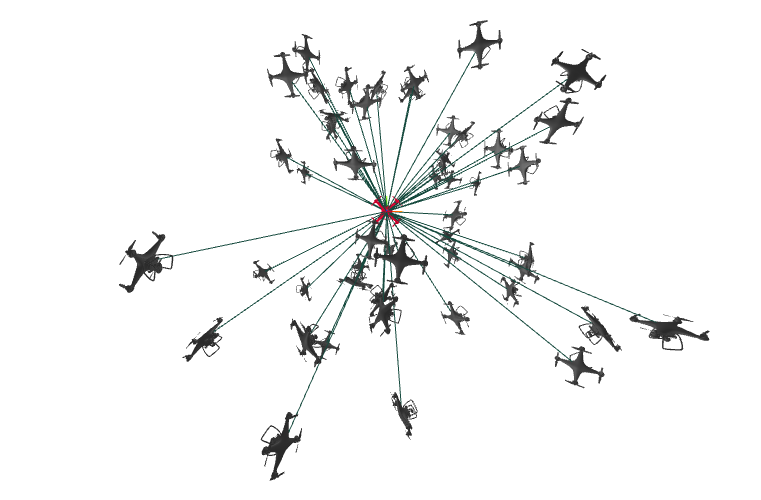
\includegraphics[width=\textwidth,height=5cm]{koopman/full_quadrotor_test_linear_trajectories.png}
		\caption{Generated point-to-point trajectories and initial conditions for testing
		tracking MPC of 6-DOF quadrotor.}
		\label{fig:rex_full_quadrotor_initial_conditions}
	\end{subfigure}
	\hfill
	\begin{subfigure}[t]{0.49\textwidth}
		\raggedright
		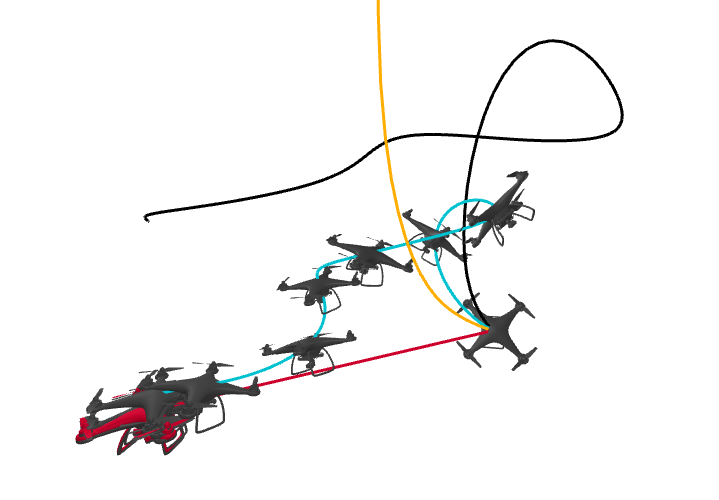
\includegraphics[width=\textwidth, height=5cm]{koopman/jdmd_full_quad_pointtopoint_with_waypoints.png}
		\caption{Performed trajectories of nominal MPC (black), EDMD (\color{orange}
		orange\color{black}), and JDMD (\color{cyan} cyan\color{black}) for tracking infeasible,
		point-to-point trajectory (\color{red} red\color{black}).}
		\label{fig:jdmd_full_quad_pointtopoint_with_waypoints}
		% \includegraphics[width=\textwidth,height=5cm]{rex_planar_quadrotor_lqr_error_by_training_window.tikz}
		% \label{fig:rex_planar_quadrotor_lqr_error_by_training_window}
	\end{subfigure}
	\caption{Point-to-point, test trajectory generation and example tracking performance of full, 6-DOF quadrotor. The test                trajectories generated include a wide scope of initial conditions beyond that of the training set, such as high                 position offset, large velocities, and near-inverted attitude. JDMD often had the best tracking performance while               successfully reaching the goal state, with a similar success rate as nominal MPC within a tighter distribution. 
	}
	% \label{fig:training_window}
\end{figure}

% %%%%%%%%%%%%%%%%%%%%%%%%%%%%%%%%%%%%%%%%%%%%%
% \subsection{Lifted versus Projected MPC}
% %%%%%%%%%%%%%%%%%%%%%%%%%%%%%%%%%%%%%%%%%%%%%

% We performed a simple experiment to highlight the value of the proposed ``projected'' MPC,
% outlined in Section \ref{sec:projected_mpc}. We trained EDMD and JDMD models with an
% increasing number of training trajectories, and recorded the first sample size at which the
% ``lifted'' and ``projected'' MPC controllers consistently stabilized the system (i.e.
% stabilized 95\% of the test initial conditions for the cartpole system for that sample size
% and subsequent ones).  The results are summarized in Table \ref{tab:mpc_comp}. The results
% quantitatively show what we qualitatively observed while training and testing these various
% examples: the projected MPC approach usually required far fewer samples to ``train'' and
% usually had better performance than its lifted counterpart that used the bilinear
% lifted dynamics. This was especially pronounced when combined with the proposed JDMD
% approach, which makes sense given that the approach explicitly encourages these Jacobians to
% match the analytical ones, so quickly converges to reasonable values with just a few training
% examples.

% \begin{wraptable}{r}{5.0cm}
%   \vspace{-2\baselineskip}
%   \begin{tabular}{ccc}\\
%     \toprule  
%     MPC       & {\color{orange} \textbf{EDMD}} & {\textbf{\color{cyan} JDMD}} \\
%     \midrule
%     Lifted    & 17   &          15 \\
%     Projected & 18   &  \textbf{2} \\
%     \bottomrule
%   \end{tabular}
%   \caption{Training trajectories required to beat nominal MPC}
%   \vspace{-1\baselineskip}
%   \label{tab:mpc_comp}
% \end{wraptable} 

\subsection{Sensitivity to Model Mismatch}

While we've introduced a significant amount of model mismatch in all of the examples so far,
a natural argument against model-based methods is that they're only as good as your model is
at capturing the salient dynamics of the system.  We investigated the effect of increasing
model mismatch by incrementally increasing the Coulomb friction coefficient between the cart
and the floor for the cartpole stabilization task (recall the nominal model assumed zero
friction). The results are shown in Table \ref{tab:friction_comp}. As expected, the number
of training trajectories required to find a good stabilizing controller increases for the
proposed approach. We achieved the results above by setting $\alpha = 0.01$, corresponding 
to a decreased confidence in our model, thereby placing greater weight on the experimental 
data. The standard EDMD approach always required more samples, and was unable to find a good
enough model above friction values of 0.4. While this could likely be remedied by adjusting
the nonlinear mapping $\phi$, the proposed approach works well with the given bases.  Note
that the nominal MPC controller failed to stabilize the system above friction values of 0.1,
so again, we demonstrate that we can improve MPC performance substantially with just a few
training samples by combining analytical gradient information and data sampled from the true
dynamics.

\begin{table}[t]
  \centering
  \begin{tabular}{cccccccc}
  \toprule 
  Friction ($\mu$) & 0.0 & 0.1 & 0.2 & 0.3 & 0.4 & 0.5 & 0.6 \\
  \midrule 
  Nominal & \cmark & \cmark & \xmark & \xmark & \xmark & \xmark & \xmark \\
  EDMD & 3 & 19 & 6 & 14 & \xmark & \xmark & \xmark \\
  JDMD & 2 & 2 & 2 & 2 & 3 & 7 & 12 \\
  \end{tabular}
  \caption{Training trajectories required to stabilize the cartpole with the given friction
    coefficient
  }
  \label{tab:friction_comp}
\end{table}

\begin{figure}[t] \centering
    \begin{subfigure}{.48\linewidth}
        \centering
		%\includegraphics[width=\textwidth,height=4.5cm]{airplane_model_error_by_alpha.tikz}
		\includegraphics[width=\textwidth,height=4cm]{koopman/airplane_model_error_by_alpha_just_jdmd.tikz}
		\caption{\changed{Median JDMD model prediction error (open-loop) and MPC tracking error (closed-loop) for perching       airplane over varying $\alpha$ values. Closed-loop behavior changes little with respect to open-loop                     prediction error. The missing open-loop values are points there the states of the open-loop system diverged              to infinity.}}
        \label{fig:model_error_alpha}
    \end{subfigure}%
    \hfill
    \begin{subfigure}{.48\linewidth}
        \centering
        \includegraphics[width=\textwidth, height=4cm]{koopman/airplane_jacobian_error.tikz} 
        \caption{\changed{Error from true model Jacobians for the  nominal model, EDMD, and JDMD. With just a few training trajectories, JDMD closely matches the Jacobian information from the nominal model. Even with  substantial training data EDMD has significant error in the Jacobians.}}
        \label{fig:airplane_jacobian_error}
    \end{subfigure}\\[1ex]
    \par\medskip
    \begin{subfigure}{\linewidth}
        \centering
        \includegraphics[width=0.6\textwidth,height=4cm]{koopman/airplane_error_by_num_train.tikz}
        \caption{\changed{Sample efficiency for the airplane perching problem.
        JDMD learns the model with only 10 training trajectories, whereas EDMD
        requires about 35. Both models perform significantly better than nominal
        MPC due to significant model mismatch at high angles of attack.}}
        \label{fig:airplane_sample_efficiency}
    \end{subfigure}
    \caption{\changed{Results on the airplane perching task}}
    % \label{fig:test}
\end{figure}

%%%%%%%%%%%%%%%%%%%%%%%%%%%%%%%%%%%%%%%%%%%%%
\subsection{Model Prediction Error vs. Controller Performance}
%%%%%%%%%%%%%%%%%%%%%%%%%%%%%%%%%%%%%%%%%%%%%

Much of the previous literature on model learning focuses on open-loop dynamics
prediction error. While intuitive, we argue that this is a poor metric when the
end goal is closed-loop control performance. In Figure
\ref{fig:model_error_alpha} we show that decreasing confidence in the analytical
model (by increasing $\alpha$) increases open-loop dynamics prediction error
significantly while having minimal impact on closed loop performance below
$\alpha = 0.7$. We found we can often quickly find models ``good enough'' for
control with just a few training trajectories (typically with a higher value of
$\alpha$), that predicted the open-loop dynamics very poorly. For example, in
Fig. \ref{fig:model_error_alpha} at the extremes of $\alpha = 0$ (EDMD) and 
$\alpha \geq 0.8$, the open-loop predictions were unstable and diverged, while
the closed-loop system still successfully tracked the reference trajectory. This
also extends to the MLP example, where MPC tracking performance does not
correlate to minimizing loss in the training and test process as seen in Fig.
\ref{fig:cartpole_train}. In addition, JDMD matches the Jacobians of that of the
nominal model (which has some Jacobian error from the true model), while EDMD
has significant Jacobian error as shown in Fig.
\ref{fig:airplane_jacobian_error}. This further demonstrates the importance of
Jacobians over open-loop dynamics prediction in a closed-loop control setting,
which may be unsurprising due to the presence of the Jacobians in the
feedback-policy of closed-loop controllers. 

%%%%%%%%%%%%%%%%%%%%%%%%%%%%%%%%%%%%%%%%%%%%%%%%%%%%%%%%%%%%%%%%%%%%%%%%%%%%%%%%%%%%%%%%%%
% Limitations 
%%%%%%%%%%%%%%%%%%%%%%%%%%%%%%%%%%%%%%%%%%%%%%%%%%%%%%%%%%%%%%%%%%%%%%%%%%%%%%%%%%%%%%%%%%
\section{Limitations} \label{sec:limitations}

\changed{Many of the limitations of the proposed approach derive from the
limitations of Koopman approaches more broadly. Foremost among these is the
sensitivity of performance to the selections of the nonlinear mapping and
respective unlifting operation; the current study has not investigated the
incorporation of the proposed method in methods which jointly learn both the 
model and the nonlinear mapping, although the extension should be fairly
straightforward.  In addition, the bilinear Koopman model assumes the original,
nonlinear dynamics to be control-affine, limiting its application to broad
dynamical systems in general.  Another significant limitation of the current
work is lack of demonstration on hardware, something we plan to remedy in the
future. Better, in-depth comparisons of the given approach to other approaches
beyond a simple MLP would also be enlightening, which were left out due to scope
limitations. Additionally, while the presented single rigid-body systems such as
a quadrotor or airplane have similar dimensionality to many autonomous systems
of interest, extensions to systems with many degrees of freedom may be difficult
computationally, given derivative information grows with the square of the state
dimension.  In addition, the relationship between closed-loop performance and
open-loop dynamics prediction error should be studied futher, given we have
demonstrated good MPC performance that has not translated directly to model
prediction error.} As with most data-driven techniques, it is difficult to claim
that our method will increase performance in all cases. It is possible that
having an extremely poor prior model may hurt rather than help the training
process. However, we found that even when the $\alpha$ parameter is extremely
small (placing little weight on the Jacobians during the learning process), it
still dramatically improves the sample efficiency over standard EDMD. It is also
quite possible that the performance gaps between EDMD and JDMD shown here can be
reduced through better selection of basis functions and better training data
sets; however, given that the proposed approach converges to EDMD as $\alpha
\rightarrow 0$, we see no reason to not adopt the proposed methodology and
simply tune $\alpha$ based on the confidence of the model and the quantity (and
quality) of training data. 

%%%%%%%%%%%%%%%%%%%%%%%%%%%%%%%%%%%%%%%%%%%%%%%%%%%%%%%%%%%%%%%%%%%%%%%%%%%%%%%%%%%%%%%%%%
% Conclusion 
%%%%%%%%%%%%%%%%%%%%%%%%%%%%%%%%%%%%%%%%%%%%%%%%%%%%%%%%%%%%%%%%%%%%%%%%%%%%%%%%%%%%%%%%%%
\section{Conclusions and Future Work} \label{sec:koopman_conclusion}

We have presented JDMD, a simple but powerful extension to EDMD that
incorporates derivative information from an approximate prior model. We have
tested JDMD in combination with a simple linear MPC control policy across a
range of systems and tasks, and have found that the resulting combination can
dramatically increase sample efficiency over EDMD, often improving over a
nominal MPC policy with just a few sample trajectories. \changed{We also showed
that the proposed approach is more efficient than a simple multi-layer
perception by one or two orders of magnitude.} Substantial areas for future work
remain: most notably, demonstrating the proposed pipeline on hardware.
Additional directions include \changed{applications on sytems with many degrees
of freedom such as those whose dynamics are governed by discretized PDEs},
lifelong learning or adaptive control applications, combining simulated and real
data through the use of modern differentiable physics engines
\cite{todorov_MuJoCo_2012,howell_Dojo_2022}, residual dynamics learning, as well
as the development of specialized numerical methods for solving nonlinear
optimal control problems using the learned bilinear dynamics.


\end{document}
